\documentclass{article}
\usepackage{polski}
\usepackage[T1]{fontenc}
\usepackage[utf8x]{inputenc}
\usepackage{booktabs}
\usepackage{multirow}
\usepackage{graphicx}
\usepackage{textcomp}
\usepackage{eurosym}
\usepackage{float}
\usepackage{adjustbox}
\usepackage{graphics}
\usepackage{tabularx}
\usepackage{rotating}
\usepackage{tabulary}
\usepackage{listings}
\usepackage{amstext}
\usepackage{xcolor}
\usepackage{url,textcomp}
\usepackage{amssymb}
\usepackage{tikz}
\usepackage{subfig}
\usepackage{graphicx}
\usepackage[document]{ragged2e}

\setlength{\voffset}{-0.5in}
\setlength{\textheight}{600pt} 

\title{SCR - Sieci Komputerowe - Laboratorium - Projekt}

\author{Damian Ryś 252936, Jakub Nowek 252889}

 
\begin{document}

\maketitle
\centering
\bfseries Grupa lab: E13-01m	

Termin zajęć: CZW 15:15-16:45 TP

Prowadzący: Dr inż. Jerzy Greblicki\\
\mdseries
\tableofcontents
\newpage
\justify

\section{Konfiguracja Adresów IP }
Zadanie polegało na odpowiednim skonfigurowaniu komputerów A,B,R tak aby były w stanie pingować siebie nawzajem. W tym celu
ręcznie konfigurujemy na każdym z nich adres IPv4 oraz dodajemy je do tej samej sieci wewnętrznej w ustawieniach virtualBoxa. Rezultaty ćwiczenia widoczne są na poniższych zrzutach ekranu:


\begin{figure}[H]
    \centering
    \subfloat[Konfiguracja komputera R.]{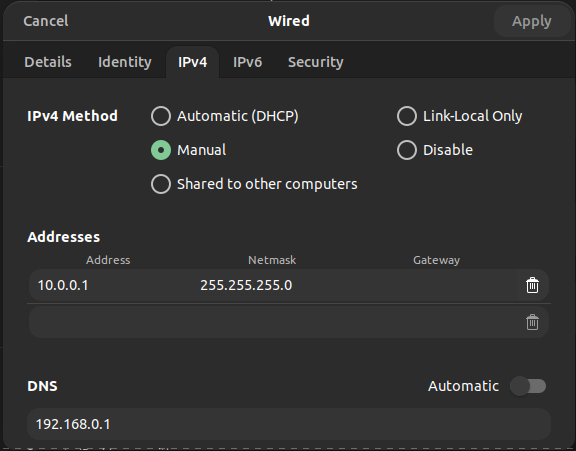
\includegraphics[width=0.5\textwidth]{1.IP/VirtualBoxVM_27pxm6gNnu.png}}
    \quad
    \subfloat[Konfiguracja komputera A.]{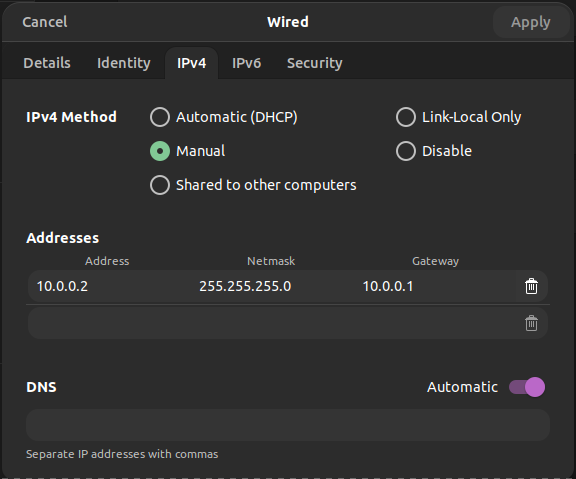
\includegraphics[width=0.45\textwidth]{1.IP/VirtualBoxVM_zHVILPyN8i.png}}
    \label{fig:my_label}
\end{figure}



\begin{figure}[H]
    \centering
    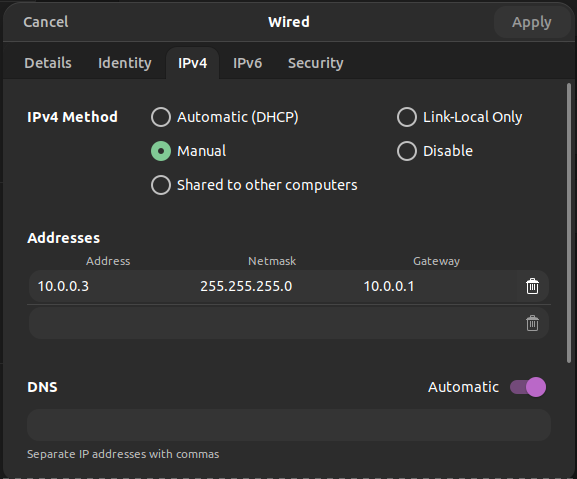
\includegraphics[totalheight=5cm]{1.IP/VirtualBoxVM_kLXjwFow7R.png}  
    \caption{Konfiguracja komputera B.}
    \label{2}
\end{figure}



\begin{figure}[H]
    \centering
    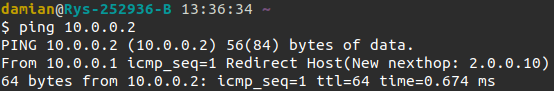
\includegraphics[totalheight=2cm]{1.IP/VirtualBoxVM_A7w5H7kGvq.png}  
    \caption{Pingowanie komputera A przy użyciu komputera B.}
    \label{2}
\end{figure}
\begin{figure}[H]
    \centering
    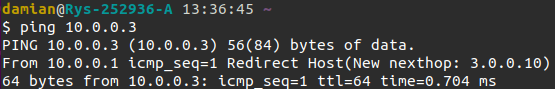
\includegraphics[totalheight=2cm]{1.IP/VirtualBoxVM_bHLFJ38p1v.png}  
    \caption{Pingowanie komputera B przy użyciu komputera A.}
    \label{2}
\end{figure}
\begin{figure}[H]
    \centering
    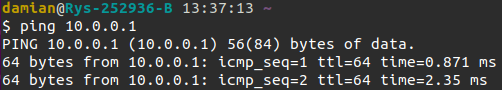
\includegraphics[totalheight=2cm]{1.IP/VirtualBoxVM_LWctJXXX3X.png}  
    \caption{Pingowanie komputera R przy użyciu komputera B.}
    \label{2}
\end{figure}

\section{Konfiguracja Routingu }
Zadanie polegało na skonfigurowaniu routingu zewnętrznego w taki sposób, aby kommputery A i B miały dostęp do Internetu przy użyciu komputera R oraz konieczne było, aby komputer spoza sieci mógł również komunikować się z komputerami w sieci wewnętrznej. Przykłady działania zostały przedstawiono poniżej:

\begin{figure}[H]
    \centering
    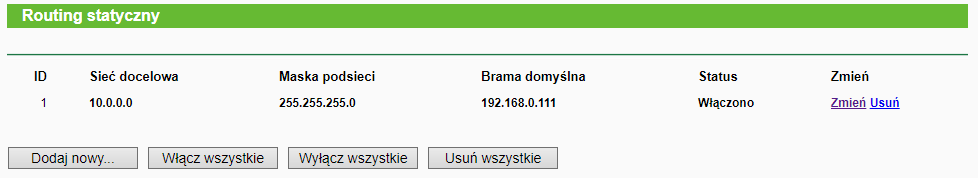
\includegraphics[totalheight=2cm]{2.Routing/opera_J2o0ex77ut.png}  
    \caption{Konfiguracja routingu zewnętrznego na routerze nadrzędnym TPlink}
    \label{2}
\end{figure}

\begin{figure}[H]
    \centering
    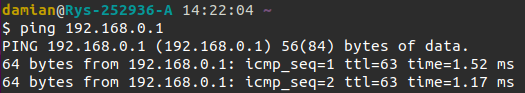
\includegraphics[totalheight=2cm]{2.Routing/VirtualBoxVM_n87Icx87hz.png}  
    \caption{Pingowanie komputera z sieci wewnętrznej do bramy domyślnej}
    \label{2}
\end{figure}

\begin{figure}[H]
    \centering
    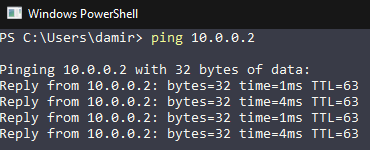
\includegraphics[totalheight=2cm]{2.Routing/powershell_V3Sz7zP30h.png}  
    \caption{Pingowanie komputera z sieci wewnętrznej do sieci zewnętrznej}
    \label{2}
\end{figure}

Aby włączyć routing na stałe, musimy zmienić opcję \textbf{ip\_forward} na \textbf{1}.

\begin{figure}[H]
    \centering
    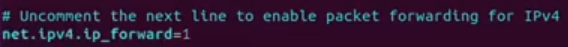
\includegraphics[totalheight=1cm]{2.Routing/wLZORom.png}  
    \caption{Plik konfiguracyjny sysctl.conf routingu.}
    \label{2}
\end{figure}

\section{Konfiguracja DHCP}
Aby uruchomić serwer DHCP należy najpierw zainstalować pakiet isc-dhcp-server.
Następnie należy otworzyć plik o tej samej nazwie w systemowym katalogu /etc/default. W linii INTERFACESV4 należy wpisać nazwę karty sieciowej serwera w sieci wewnętrznej.

\begin{figure}[H]
    \centering
    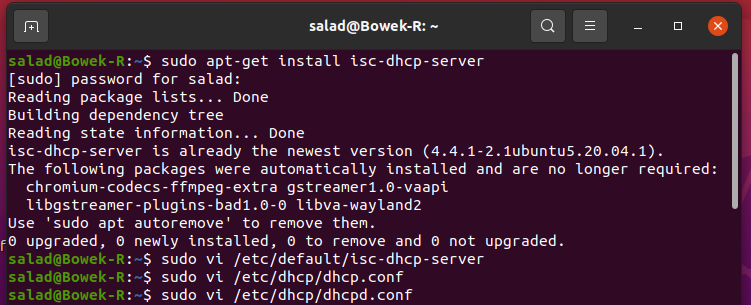
\includegraphics[scale = 0.75]{dhcp/dhcp2.png}  
    \caption{Instalowanie pakietu i komendy otwarca plików.}
    \label{2}
\end{figure}

\begin{figure}[H]
    \centering
    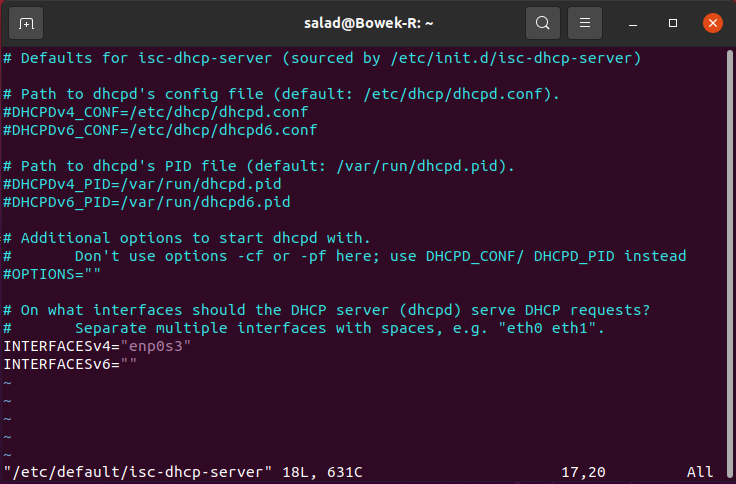
\includegraphics[scale = 0.75]{dhcp/dhcp3.png}  
    \caption{Dodawanie nazwy karty sieciowej.}
    \label{2}
\end{figure}

Potem otwieramy plik konfiguracyjny dhcpd.conf i dokonujemy w nim następujących zmian: odkomentowujemy opcję autoritative oraz konfigurację wewnętrznej podsieci, w której wpisujemy nasze adresy IP oraz wybieramy czasy dzierżawy adresów.

\begin{figure}[H]
    \centering
    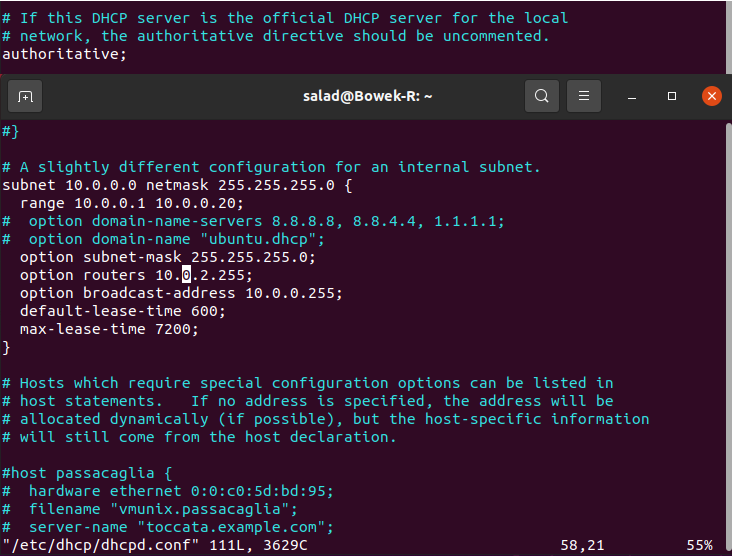
\includegraphics[scale = 0.68]{dhcp/dhcp4.png}  
    \caption{Modyfikacja pliku dhcpd.config.}
    \label{2}
\end{figure}

Teraz możemy włączyć serwer sprawdzić, czy został poprawnie aktywowany, komendami: systemctl start oraz systemctl status. Jak widać, serwer został aktywowany poprawnie. 

\begin{figure}[H]
    \centering
    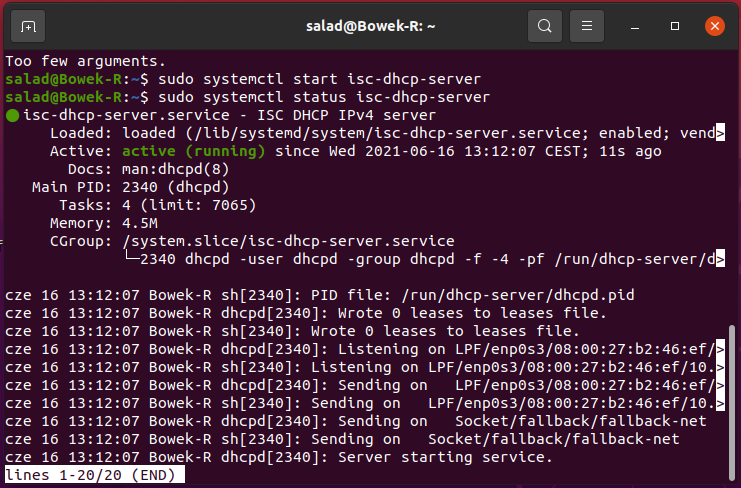
\includegraphics[scale = 0.68]{dhcp/dhcp5_dziala.png}  
    \caption{Sprawdzanie aktywności serwera.}
    \label{2}
\end{figure}

Jeśli teraz ustawimy kartę sieciową komputera B zgodnie z poniższym rysunkiem, to powinniśmy zobaczyć komputer B w komputerze R na liście komputerów dzierżawiących adres.

\begin{figure}[H]
    \centering
    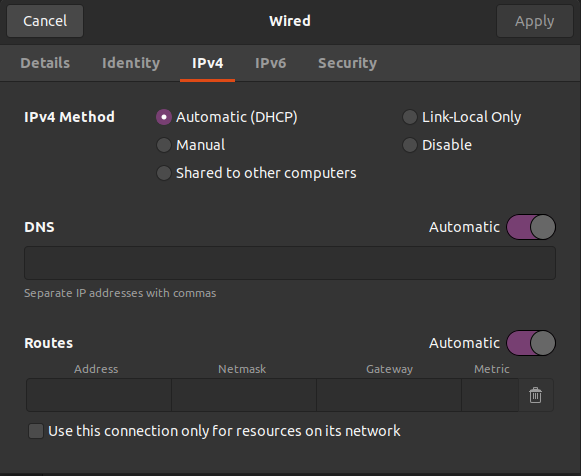
\includegraphics[scale = 0.8]{dhcp/dhcp_lease_dowody.png}  
    \caption{Ustawienia koputera B.}
    \label{2}
\end{figure}

\begin{figure}[H]
    \centering
    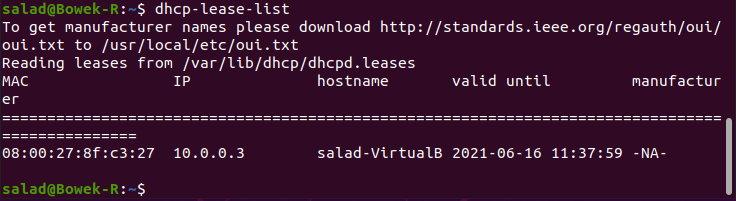
\includegraphics[scale = 0.68]{dhcp/dhcp_lease.png}  
    \caption{Lista komputerów połączonych z serwerem DHCP.}
    \label{2}
\end{figure}
\newpage
\section{Uruchomienie NAT }
Aby korzystać z usługi NAT należy dokonać mian w pliku konfiguracyjnym fireawalla /etc/ufw/before.rules, według poniższego wzoru. 

\begin{figure}[H]
    \centering
    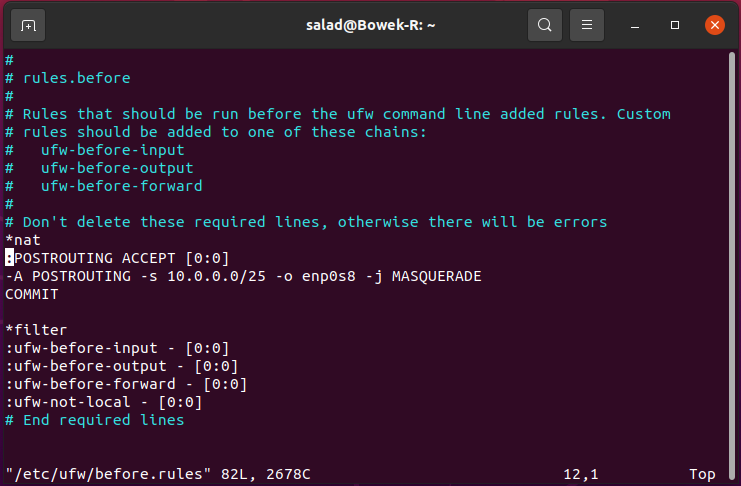
\includegraphics[scale = 0.75]{NAT/nat1.png}  
    \caption{Edytowanie pliku before.rules.}
    \label{2}
\end{figure}

\begin{figure}[H]
    \centering
    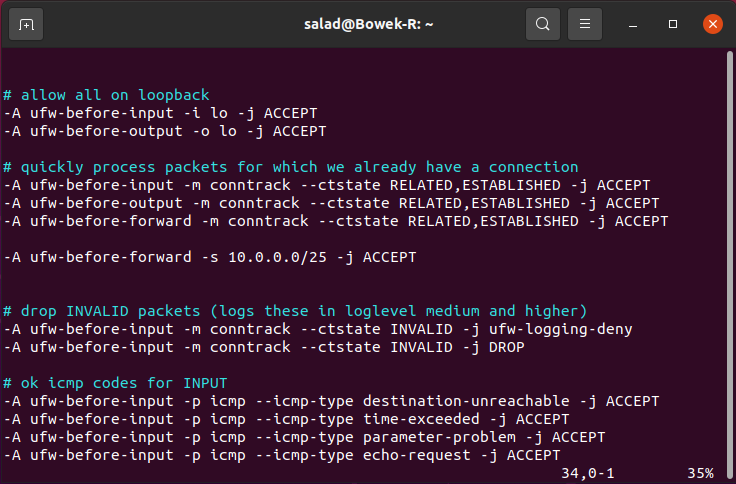
\includegraphics[scale = 0.75]{NAT/nat2.png}  
    \caption{Edytowanie pliku before.rules.}
    \label{2}
\end{figure}
\newpage
\justify
Aby sprawdzić, czy usługa działa, pingujemy adres, np 8.8.8.8 z komputera A, a następnie sprawdzamy z jakiego adresu zostało wykonane połączenie. Komputer R powinien zamienić adres wewnętrzny komputera A na swój adres zewnętrzny. Jak widać na poniższych rysunkach wszystkie operacje zostały przeprowadzone pomyślnie.
\begin{figure}[H]
    \centering
    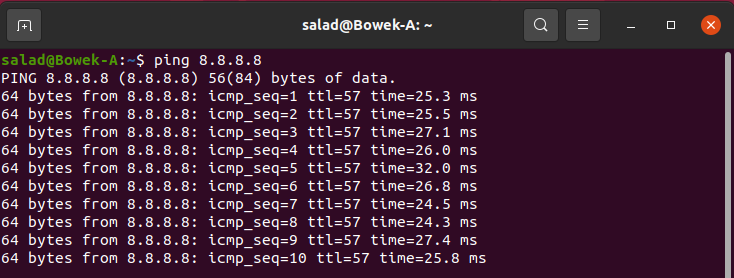
\includegraphics[scale = 0.85]{NAT/nat3A.png}  
    \caption{Pingowanie adresu Google'a z komputera A.}
    \label{2}
\end{figure}

\begin{figure}[H]
    \centering
    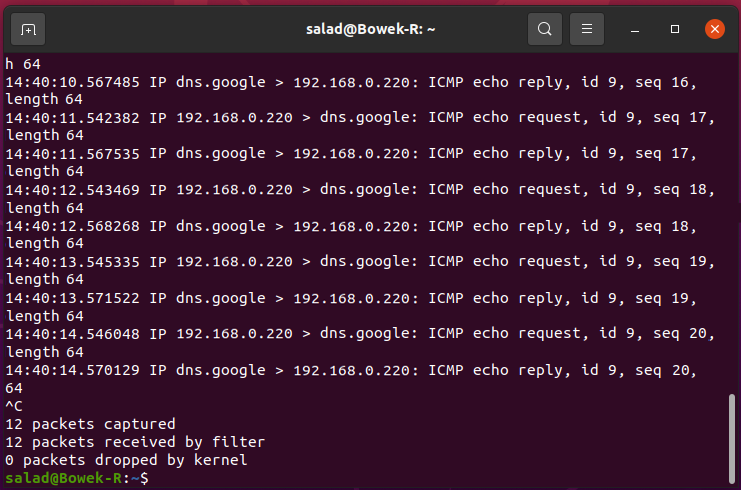
\includegraphics[scale = 0.5]{NAT/nat4.png}  
    \caption{Wykaz zapytań i odpowiedzi na komputerze R.}
    \label{2}
\end{figure}
\newpage

\section{Uruchomienie DNS i DDNS }

Dla systemu Linux powstało wiele programów pełniących funkcje severa DNS, jednakże zdecydowałem się na skorzystanie z servera BIND ze względu na duże wsparcie społeczności i jego popularność. Po zainstalowaniu wymagane było skonfigurowane klienta do korzystania z lokalnego servera DNS oraz konfiguracja domeny lokalnej. Kolejne zrzuty ekranów z plików konfiguracyjnych znajdują się poniżej:

\begin{figure}[H]
    \centering
    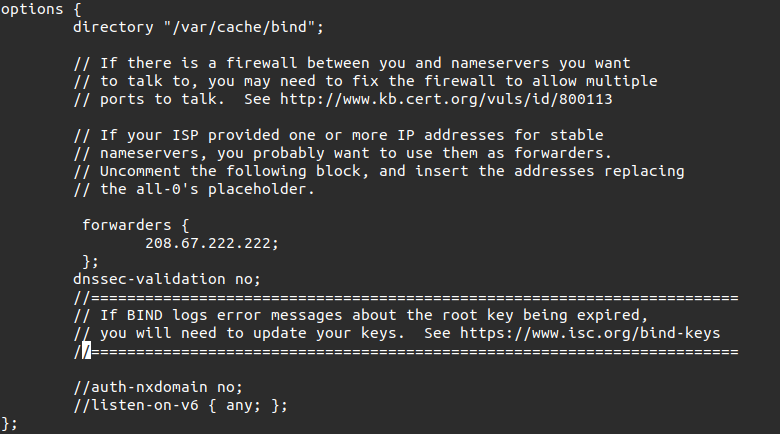
\includegraphics[scale = 0.45]{DNS/1D5i9Yw.png}  
    \caption{Skonfigurowany plik /etc/bind/named.conf.options}
    \label{2}
\end{figure}

\begin{figure}[H]
    \centering
    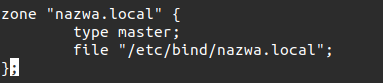
\includegraphics[scale = 0.8]{DNS/heUah3h.png}  
    \caption{Skonfigurowany plik /etc/bind/named.conf.local}
    \label{2}
\end{figure}

\begin{figure}[H]
    \centering
    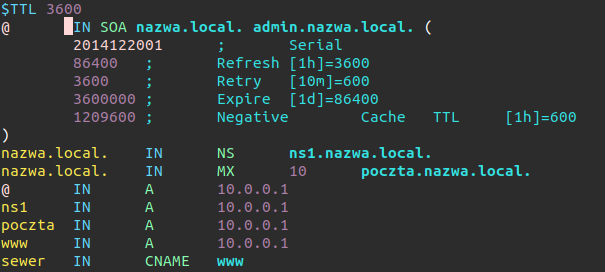
\includegraphics[scale = 0.45]{DNS/UmpPeuu.png}  
    \caption{Skonfigurowany plik /etc/bind/nazwa.local}
    \label{2}
\end{figure}



\begin{figure}[H]
    \centering
    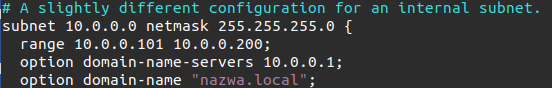
\includegraphics[scale = 0.5]{DNS/nXDSlle.png}  
    \caption{Zmiana konfiguracji DHCP}
    \label{2}
\end{figure}

\begin{figure}[H]
    \centering
    
\includegraphics[scale = 0.6]{DNS/hzcTdrj.png}  
    \caption{Skonfigurowana plik /etc/resolv.conf}
    \label{2}
\end{figure}

\begin{figure}[H]
    \centering
    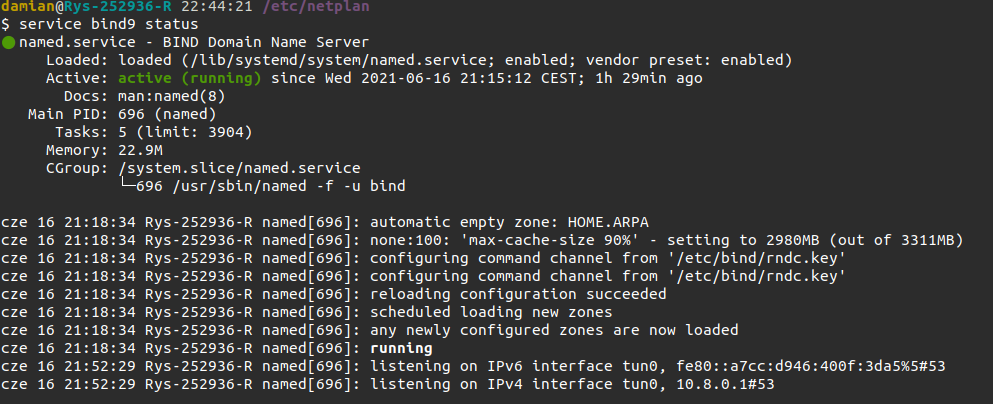
\includegraphics[scale = 0.35]{DNS/SFBDYnG.png}  
    \caption{Działąjacy server BIND }
    \label{2}
\end{figure}


\begin{figure}[H]
    \centering
    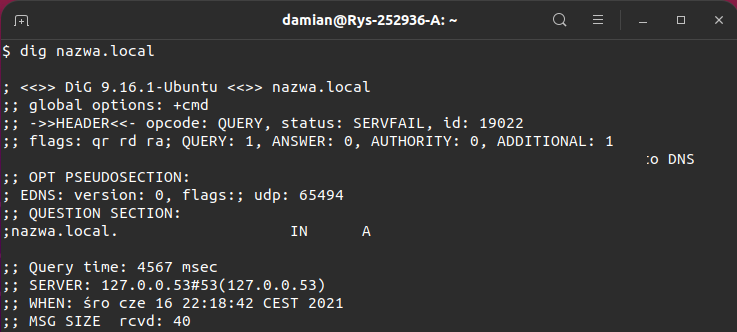
\includegraphics[scale = 0.45]{DNS/dns.png}  
    \caption{Działający server DNS po komputera A}
    \label{2}
\end{figure}
\newpage
\section{Uruchomienie VPN}
Do uruchomienia serwera VPN posłużymy się usługą openVPN. Po wstępnej konfiguracji, zainstalowano klient na głównym komputerze, na którym został zainstalowany certyfikat dostępu. Teraz można podłączyć się do nowej sieci. Kolejne kroki zostały przedstawione na rysunkach poniżej:

\begin{figure}[H]
    \centering
    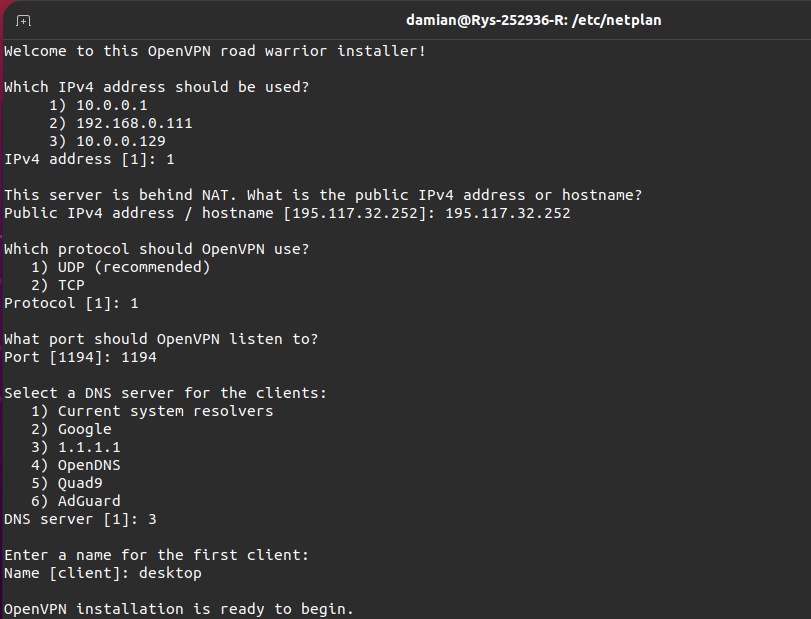
\includegraphics[scale = 0.45]{VPN/RgpW9tg.png}  
    \caption{Instalacja serwera VPN }
    \label{2}
\end{figure}

\begin{figure}[H]
    \centering
    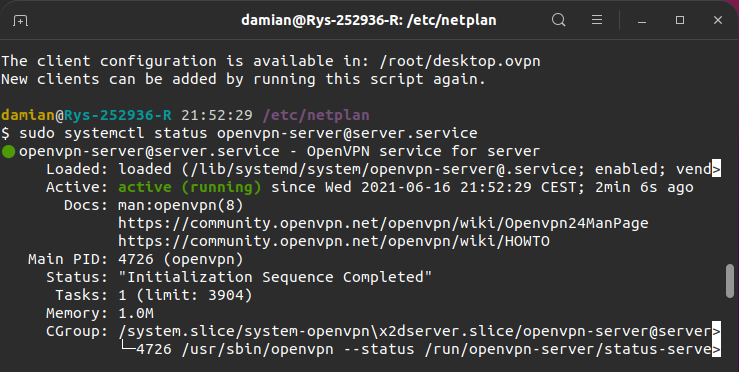
\includegraphics[scale = 0.45]{VPN/Sxo4ajG.png}  
    \caption{Dzialajacy serwer VPN }
    \label{2}
\end{figure}

\begin{figure}[H]
    \centering
    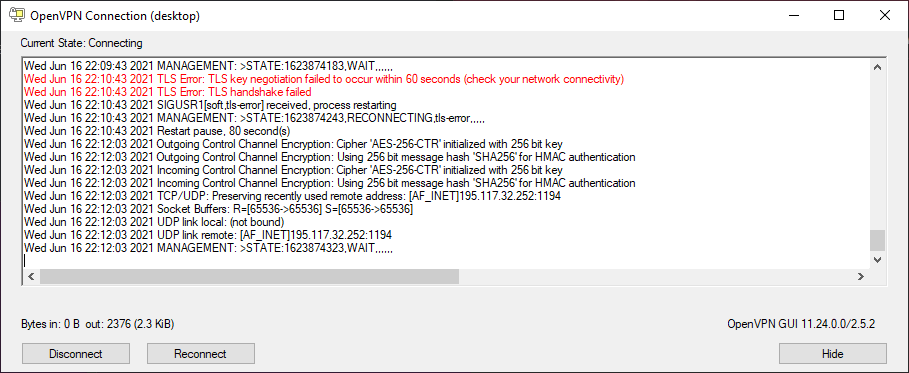
\includegraphics[totalheight = 5cm]{VPN/8AkDDvG.png}  
    \caption{Połączony klient z serverem VPN z pomocą openVPN GUI}
    \label{2}
\end{figure}

\begin{figure}[H]
    \centering
    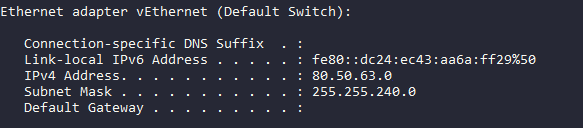
\includegraphics[scale = 0.6]{VPN/21312321.png}  
    \caption{Nowy adres IPV4 klienta}
    \label{2}
\end{figure}
\newpage
\section{Uruchomienie serwera WWW}
Do uruchomienia serwera www posłużymy się usługą Apache2. Po skonfigurowaniu usługi oraz zapory nasza usługa jest gotowa do użytku co zostało zademonstrowane poniżej:

\begin{figure}[H]
    \centering
    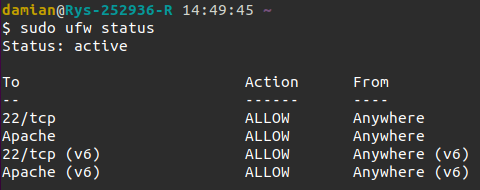
\includegraphics[totalheight=4cm]{6.WWW/2yeHK9Z.png}  
    \caption{Skonfigurowana zapora na komputerze R}
    \label{2}
\end{figure}



\begin{figure}[H]
    \centering
    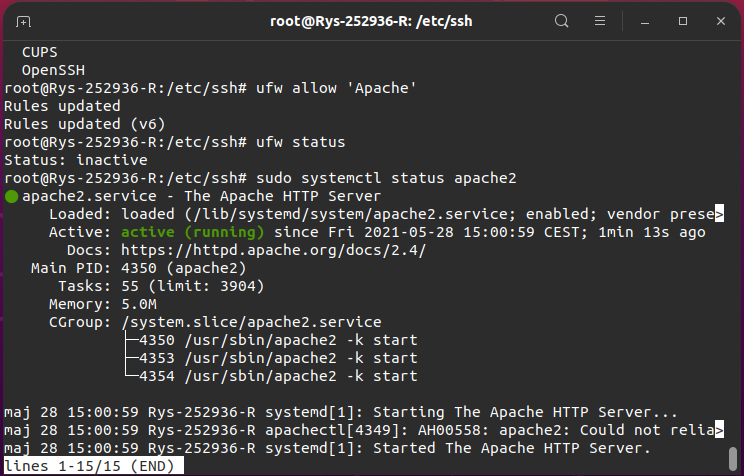
\includegraphics[totalheight=6cm]{6.WWW/VirtualBoxVM_6Um6MFTiwV.png}  
    \caption{Uruchomiony serwer WWW na komputerze R}
    \label{2}
\end{figure}

\newpage
\begin{figure}[H]
    \centering
    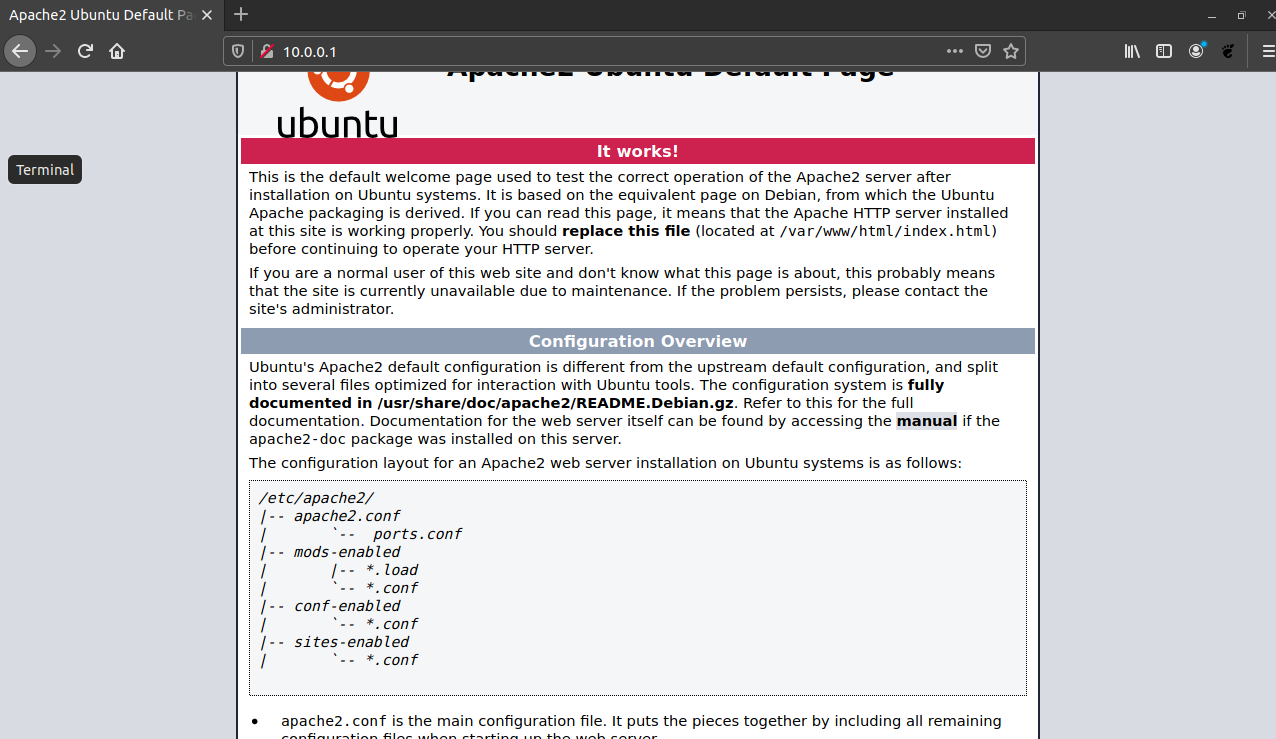
\includegraphics[totalheight=6cm]{6.WWW/VirtualBoxVM_epWXKYFWp9.png}  
    \caption{Domyślna strona www dla adresu IP komputera R}
    \label{2}
\end{figure}

\begin{figure}[H]
    \centering
    
\includegraphics[totalheight=6cm]{6.WWW/5jK32TG.png}  
    \caption{Jak widzimy stronę możemy dowolnie konfigurować}
    \label{2}
\end{figure}

\section{Uruchomienie serwera SSH}
Zadanie polegało na uruchomieniu serwera SSH na komputerze R. Serwer został skonfigurowany, aby połączenie było możliwe przy użyciu portu 2222 w celu uniknięcia kolizji portów oraz wyłączone zostały klucze SSH dla logowania dla nadrzędnego użytkownika( logujemy się normalnie poprzez hasło). Poniżej znajduję się zademonstrowanie działającej usługi:
\newpage
\begin{figure}[H]
    \centering
    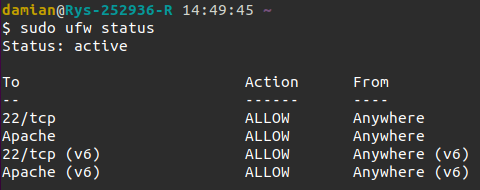
\includegraphics[scale = 0.72]{6.WWW/2yeHK9Z.png}  
    \caption{Skonfigurowana zapora na komputerze R}
    \label{2}
\end{figure}

\begin{figure}[H]
    \centering
    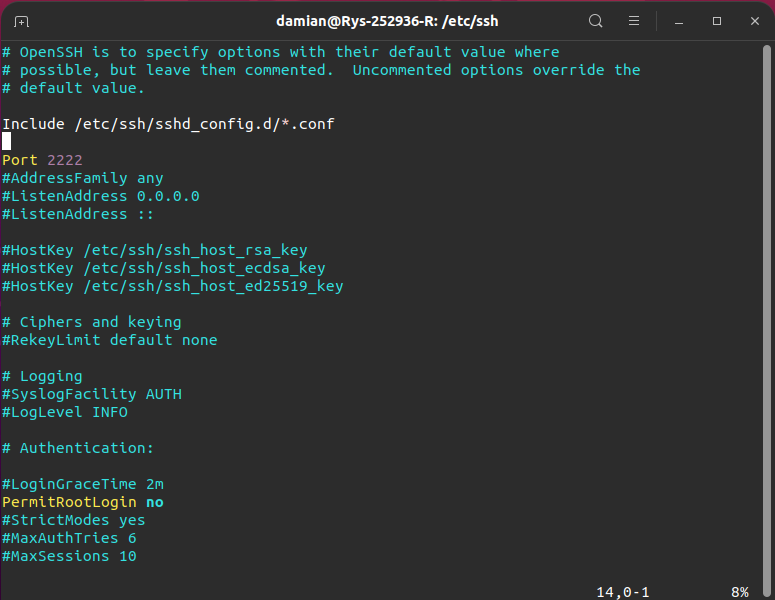
\includegraphics[scale = 0.45]{7.SSH/TWO3cUq.png}  
    \caption{Konfiguracja pliku sshd\_config na komputerze R}
    \label{2}
\end{figure}

\newpage
\begin{figure}[H]
    \centering
    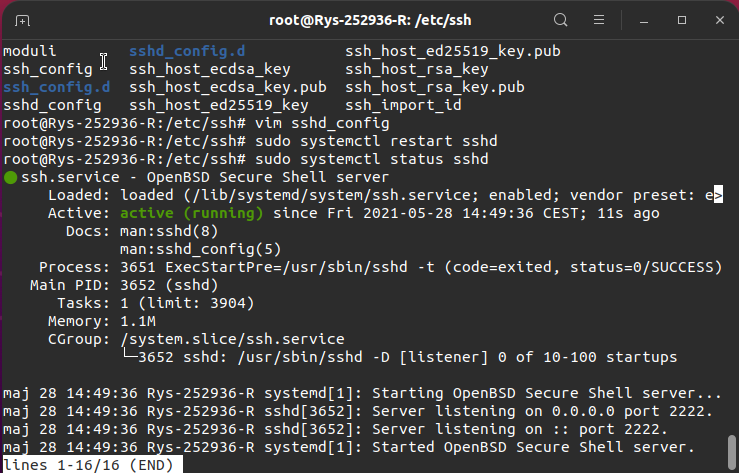
\includegraphics[scale = 0.65]{7.SSH/VirtualBoxVM_6noF4O3CM7.png}  
    \caption{Uruchomiony server SSH na komputerze R}
    \label{2}
\end{figure}

\begin{figure}[H]
    \centering
    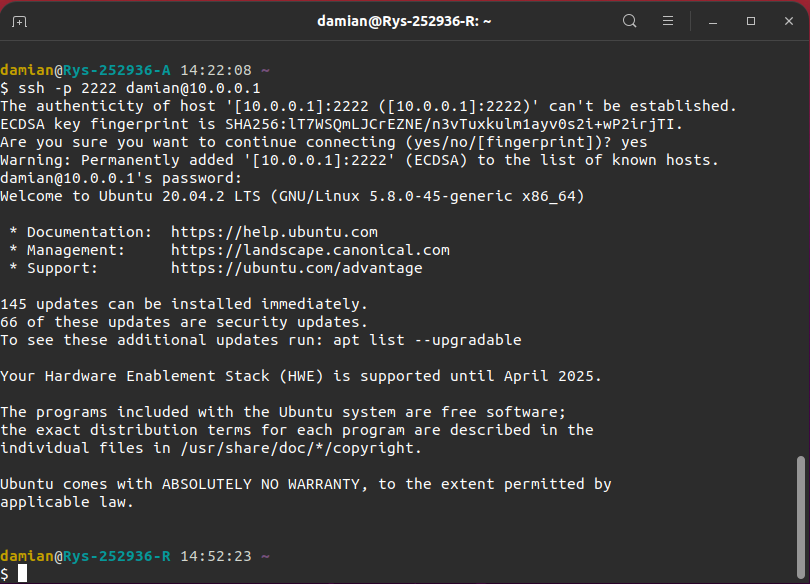
\includegraphics[scale = 0.6]{7.SSH/VirtualBoxVM_6umd4MDHVJ.png}  
    \caption{Logowanie do servera R przy użyciu komputera A}
    \label{2}
\end{figure}

\newpage
\section{Uruchomienie serwera FTP}
Zadanie polegało na uruchomieniu serwera FTP na komputerze R, tak by komputery A i B miały dostęp do plików na nim udostępnionych.

Na początku należy zainstalować vsftpd oraz sprawdzić czy usługa została poprawnie zainstalowana, komendą service vsftpd status.
\begin{figure}[H]
    \centering
    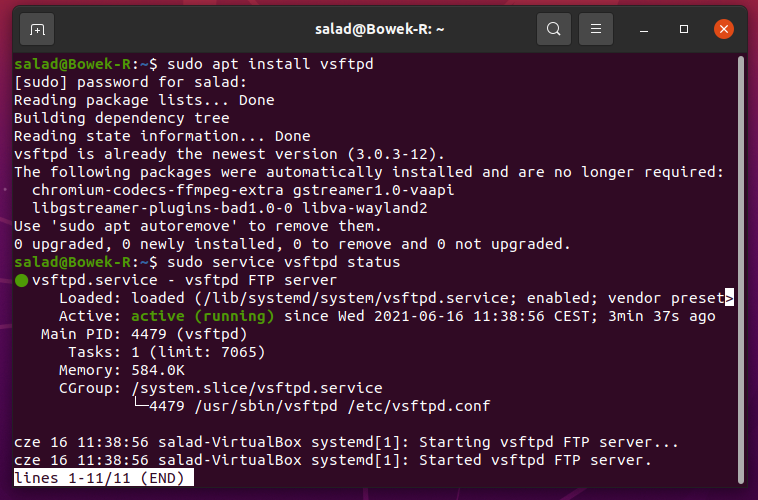
\includegraphics[scale = 0.65]{ftp/FTP_1.png}  
    \caption{Instalowanie vsftpd.}
    \label{3}
\end{figure}

Następnie należało uaktywnić porty komendą ufw allow, a następnie sprawdzić, czy zostały poprawnie aktywowane komendą ufw status.

\begin{figure}[H]
    \centering
    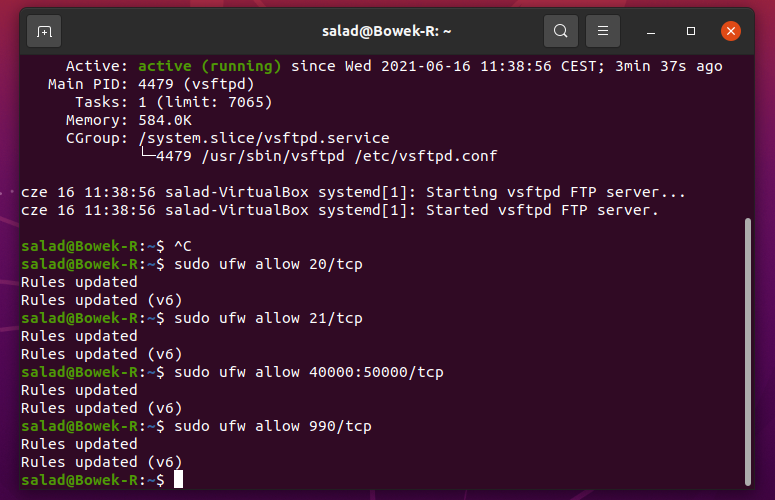
\includegraphics[scale = 0.65]{ftp/ftp_porty.png}  
    \caption{Otwieranie portów.}
    \label{4}
\end{figure}

\newpage
\begin{figure}[H]
    \centering
    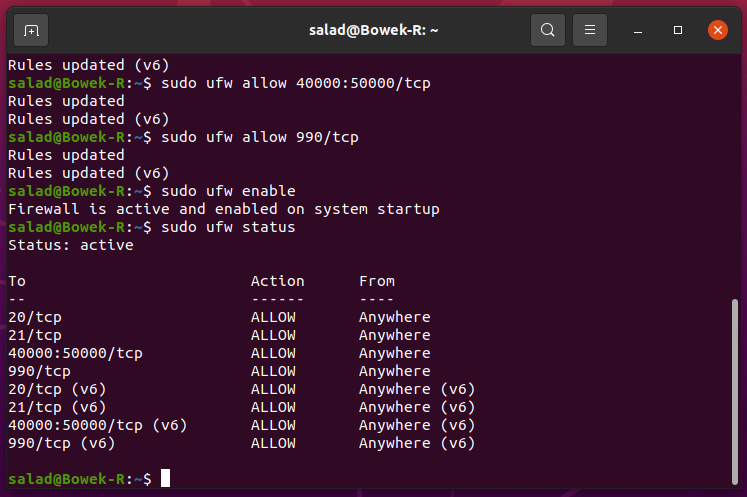
\includegraphics[scale = 0.65]{ftp/ftp_active.png}  
    \caption{Sprawdzanie stanu portów.}
    \label{5}
\end{figure}

Potem dodajemy użytkownika serwera.

\begin{figure}[H]
    \centering
    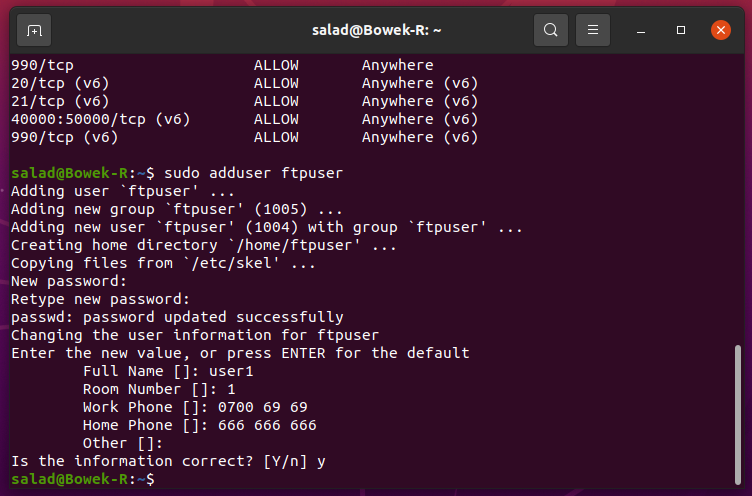
\includegraphics[scale = 0.65]{ftp/ftp_adduser.png}  
    \caption{Dodawanie użytkownika serwera FTP.}
    \label{5}
\end{figure}
\justify

Następnie dla użytkownika zostały stworzony folder w którym może przechowywać pliki. Ścieżka do folderu plików użytkownika: /home/ftpuser/ftp/files.
\newpage
\begin{figure}[H]
    \centering
    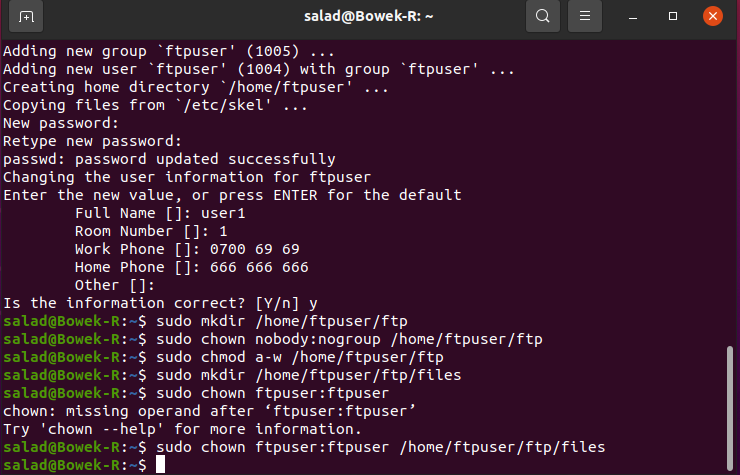
\includegraphics[scale = 0.65]{ftp/ftp_usser.png}  
    \caption{Dodawanie katalogu użytkownika.}
    \label{5}
\end{figure}
\justify
Stworzony został również plik w folderze etc, do przechowywania konfiguracji serwera.

\begin{figure}[H]
    \centering
    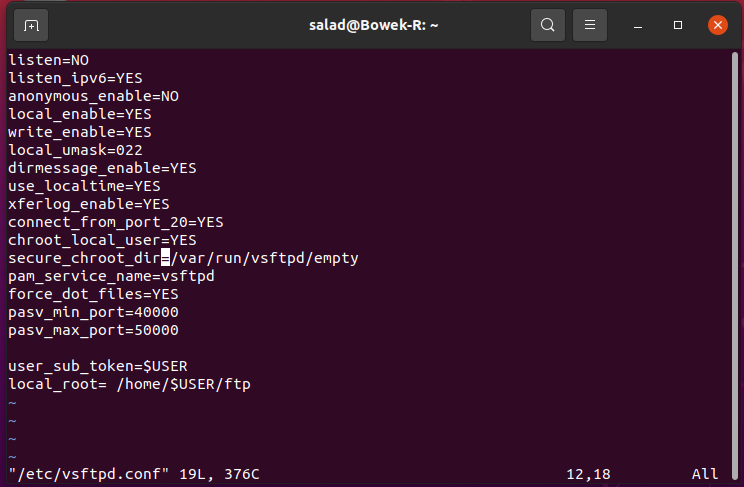
\includegraphics[scale = 0.65]{ftp/ftp_conf.png}  
    \caption{Plik konfiguracyjny.}
    \label{5}
\end{figure}
\justify
Po tych czynnościach serwer jest gotowy do użytku. Teraz można wrzucić na niego jakiś plik z komputera R i sprawdzić, czy uzyskamy do niego dostęp na komputerze A. Plik możemy przenieść do folderu użytkownika za pomocą komend lub tak jak w przykładzie, za pomocą programu Filezilla. Aby za pomocą Filezilli połączyć się z serwerem, w polach u góry podajemy adres IP hosta w wewnętrznej sieci 10.0.0.1, nazwę użytkownika oraz hasło. Jak widać na poniższym rysunku, plik został poprawnie przeniesiony na serwer.
\newpage
\begin{figure}[H]
    \centering
    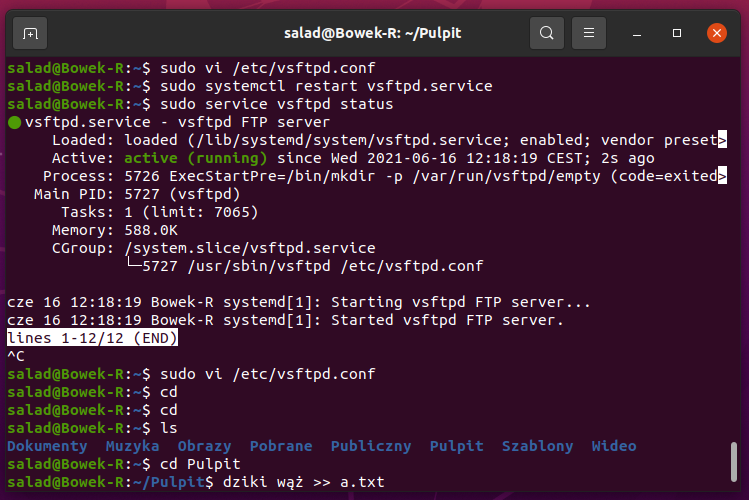
\includegraphics[scale = 0.7]{ftp/running.png}  
    \caption{Tworzenie pliku.}
    \label{5}
\end{figure}

\begin{figure}[H]
    \centering
    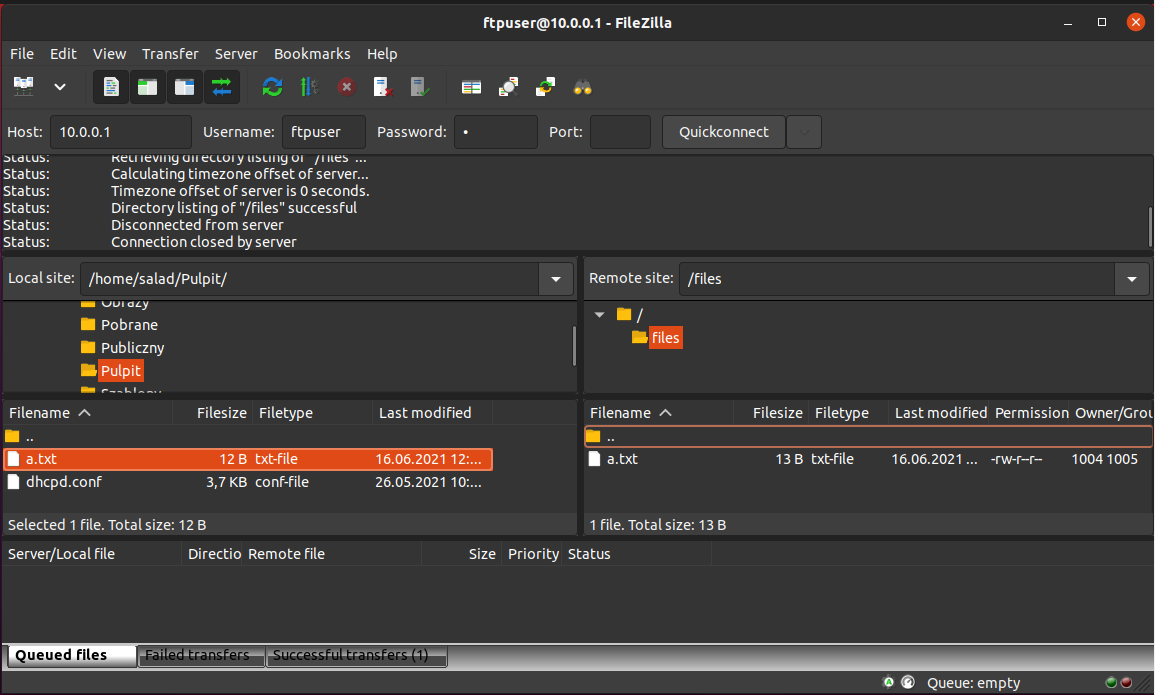
\includegraphics[scale = 0.45]{ftp/filezilla.png}  
    \caption{Wrzucanie pliku na serwer.}
    \label{5}
\end{figure}
Teraz można sprawdzić od strony terminala, czy plik został poprawnie wrzucony. Jak widać poniżej, plik znajduje się w folderze files. Z serwerem łączymy się wpisując komendę z adrese serwera: ftp 10.0.0.1 .
\newpage
\begin{figure}[H]
    \centering
    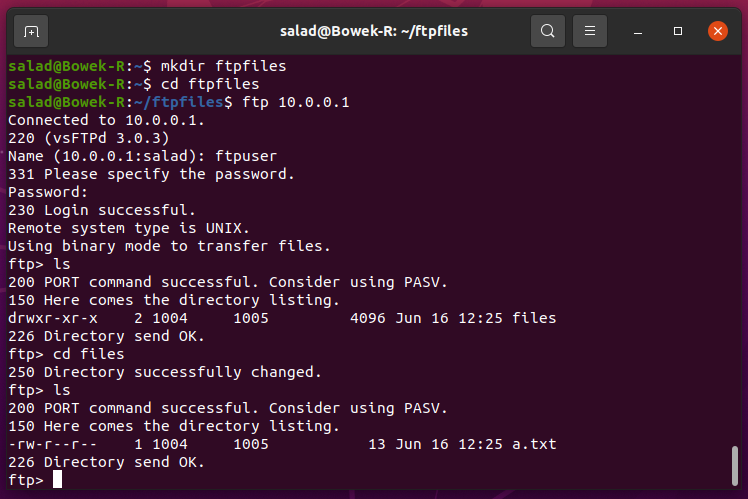
\includegraphics[totalheight=6cm]{ftp/logowanie_i_pliki.png}  
    \caption{Plik poprawnie umieszczony w folderze files.}
    \label{5}
\end{figure}

Teraz sprawdzamy dostęp do tego serwera z komputera A. Komputer A łączymy z serwerem komendą ftp 10.0.0.1, a następnie wchodzimy w folder z plikiem i pobieramy go przy użyciu komendy get. Jak widać na poniższym rysunku, plik został pomyślnie pobrany i umieszczony w folderze domowym na komputerze A.

\begin{figure}[H]
    \centering
    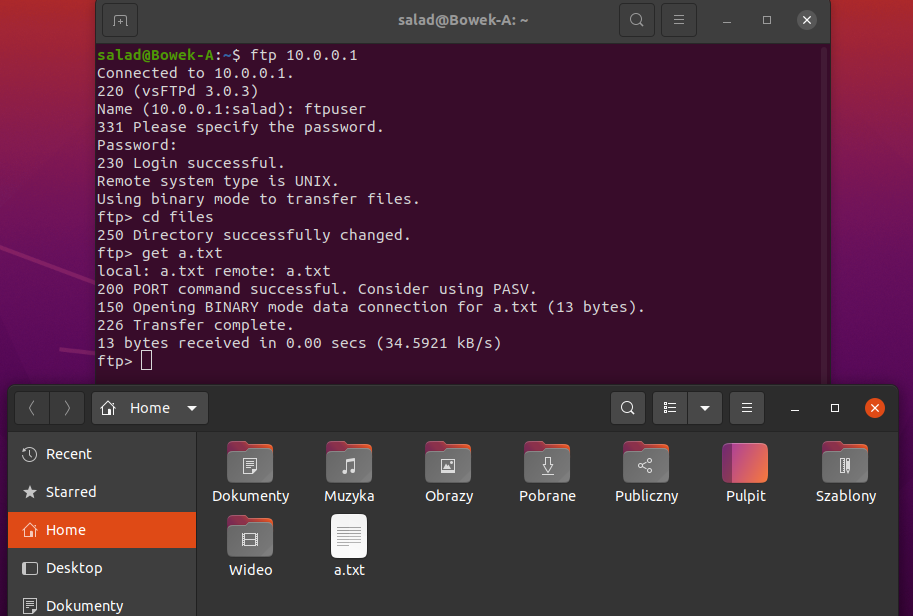
\includegraphics[totalheight=6cm]{ftp/dziala_dowody.png}  
    \caption{Pobieranie pliku z serwera na komputer A.}
    \label{5}
\end{figure}



\section{Wnioski}
Wszystkie omówione i zaprezentowane usługi działają poprawnie. Należy jednak pamiętać, o poprawnej konfiguracji routera łączącego nas z siecią zewnętrzną oraz o poprawnej konfiguracji maszyn wirtualnych wykorzystanych w zadaniach.
\end{document}